%%% LaTeX Template: Article/Thesis/etc. with colored headings and special fonts
%%%
%%% Source: http://www.howtotex.com/

\documentclass[12pt]{article}


\usepackage{apuntes-estilo}
\usepackage{fancyhdr,lastpage}
\usepackage{color,colortbl}
\usepackage{verbatim}

\def\maketitle{

% Titulo 
 \makeatletter
 {\color{bl} \centering \huge \sc \textbf{
 Particionado y sistema de archivos \\ 
\large \vspace*{-8pt} \color{black} Guia básica sobre particionado y sistema de archivos.
 \vspace*{8pt} }\par}
 \makeatother


% Autor
 \makeatletter
 {\centering \small 
 	Departamento de Ingeniería de Computadoras \\
 	Facultad de Informática - Universidad Nacional del Comahue \\
 	\vspace{20pt} }
 \makeatother

}

% Custom headers and footers
\fancyhf{} % clear all header and footer fields
\fancypagestyle{plain}{\fancyhf{}}
  	\pagestyle{fancy}
 	\lhead{\footnotesize Particionado y sistema de archivos - Departamento de Ingeniería de Computadoras}
 	\rhead{\footnotesize \thepage\ }	% ''Page 1 of 2''

\def\ti#1#2{\texttt{#1} & #2 \\ }



\begin{document}

\thispagestyle{empty}
\maketitle
\setlength{\parindent}{0pt}

\section*{Introducción}

Las actividades sobre los medios masivos de almacenamiento son altamente 
frecuentes dentro de las tareas de los administradores. La administración 
del espacio de almacenamiento (datos), involucra varias tareas: diseño 
del uso de discos, particionado para ajustarse al diseño, creación de 
sistema de archivos que permitan organizar la información dentro de los
discos (que de por sí no son más que una secuencia de bits sin sentido),
monitoreo del consumo de espacio, ajustes de acuerdo al uso, copias de 
respaldo en caso de fallas, entre otras. 

En este apunte se cubren los conceptos básicos de particionamiento de 
discos y sistemas de archivos.  

\section*{Particiones}

Un disco rígido puede dividirse en varias particiones.{\bf Cada partición 
funciona como si fuera un disco duro independiente.} 
La idea es que si sólo se tiene un disco, y se quieren tener, digamos,
 dos sistemas operativos en él, se pueda dividir 
el disco en dos particiones. Cada sistema operativo utilizará su propia 
partición tal y como se desea, y no tocará 
la otra. De esta forma los dos sistemas operativos pueden coexistir 
pacíficamente en un mismo disco rígido. En este ejemplo, si no tuviésemos
particiones necesitaríamos comprar un disco rígido para cada sistema 
operativo.

Además de los discos rígidos, otros dispositivos de almacenamiento 
masivo suelen particionarse, como por ejemplo las memorias flash (pendrive).Este apunte pretende cubrir el concepto de particionado, aplicando en par
ticular dicho concepto a los esquemas seguidos por las PC convencionales.  


\subsection*{El MBR, sectores de arranque y la tabla de particiones}

La información sobre cómo se particiona un disco se almacena en su primer 
sector (estos son los primeros bytes al comienzo del dispositivo, 
dependiendo del tipo de dispositivo particular es la cantidad de bytes 
que representan el primer sector). Este primer sector es el registro de 
arranque maestro (MBR, del inglés Master Boot Record) del disco; éste es 
el sector que la BIOS lee y arranca cuando se enciende la máquina. 

El esquema de partición no está integrado en el hardware, ni siquiera 
en la BIOS. Tan sólo es una convención que muchos (no todos) sistemas 
operativos siguen. Algunos sistemas operativos soportan particiones pero 
con esquemas diferentes, en muchos casos para coexistir con el esquema 
mencionado, ocupan una partición convencional en el disco duro, y 
utilizan su propio sistema de particionamiento dentro de esa partición 
(por ejemplo, esto sucede con el sistema operativo Solaris sobre 
arquitectura x86). La mayoría de los sistemas operativos modernos
soportan particionado, sin embargo es bueno tener presente que si estamos 
frente a un sistema operativo  que no lo soporta, entonces  no podrá 
coexistir en un mismo disco con los que si. 

Es importante almacenar la información detallada de las tablas de 
particiones en una computadora distinta, mediante algún mecanismo de 
copia de respaldo, para poder recuperar la información almacenada en 
caso de que la tabla de particiones sea modificada por error. En 
particular el comando \texttt{fdisk} nos permite listar esta información: 

\colorbox{grey}{\parbox[t]{0.95\linewidth}{ \vspace*{0.5cm} { 
{\bf Ejemplo : información de particiones del disco \texttt{/dev/sdb}}\\
{\tt
\#fdisk -l /dev/sdb\\
Disk /dev/sdb: 80.0 GB, 80032038912 bytes\\
255 heads, 63 sectors/track, 9730 cylinders, 156312576 sectores en total\\
Units = sectores of 1 * 512 = 512 bytes\\
Sector size (logical/physical): 512 bytes / 512 bytes\\
I/O size (minimum/optimal): 512 bytes / 512 bytes\\
Identificador del disco: 0x00005700\\
\\
Disposit. Inicio    Comienzo      Fin      Bloques  Id  Sistema\\
/dev/sdb1   *        2048    39063551    19530752   83  GNU/Linux\\
/dev/sdb2        39063552    42969087     1952768   82  GNU/Linux swap / Solaris\\
/dev/sdb3        42969088   156311551    56671232   83  GNU/Linux\\
}
} \vspace*{0.5cm} } } 

\subsection*{Particiones extendidas y lógicas}

El esquema original de particionamiento para discos duros de PC permitía 
solamente cuatro particiones. Esto rápidamente se volvió demasiado escaso 
para la vida real, en parte porque algunas personas querían más de cuatro 
sistemas operativos (Linux, MS-DOS, OS/2, Minix, FreeBSD, NetBSD, o 
Windows/NT, por nombrar algunos), pero principalmente 
porque algunas veces es buena idea tener varias particiones para un mismo 
sistema operativo. Por ejemplo, el espacio swap está generalmente mejor 
colocado para GNU/Linux en su propia partición en lugar de la partición 
principal por cuestiones de rapidez (vea más abajo). También por ejemplo 
podríamos querer limitar el espacio disponible 
para archivos de usuarios, de modo que el directorio \texttt{/home} se 
encuentre en una partición separada. 

Para superar esta limitación de diseño, se inventaron las particiones 
extendidas. Este truco permite particionar una partición primaria en 
sub-particiones. Esta partición primaria subdividida es la partición 
extendida; las sub-particiones son las particiones lógicas. Se comportan 
como particiones primarias, pero se crean de diferente manera. No existen
diferencias de rendimiento entre ellas.

La estructura de particiones de un disco duro debe parecerse a la que 
aparece en la figura a continuación. El disco se divide en tres particiones 
primarias, la segunda de las cuales se divide en dos 
particiones lógicas. Una parte del disco no está particionada. El disco 
como un todo y cada partición primaria tienen un sector de arranque.

\begin{center}
 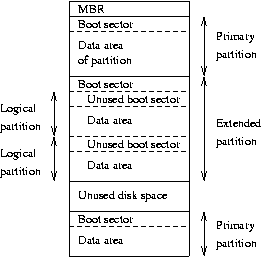
\includegraphics{hd-layout.png}
\end{center}

\subsection*{Particionando el disco duro}

Existen muchos programas para crear y eliminar particiones. La mayoría de 
sistemas operativos tienen el suyo propio, y es buena idea utilizar el 
propio con cada sistema operativo, por si se diera el caso que haga algo 
inusual que los otros no puedan hacer. Muchos de estos programas se 
llaman \texttt{fdisk}, incluido el de GNU/Linux, o variaciones de esa 
palabra. Los detalles de uso del fdisk de GNU/Linux se dan en su página 
de manual. El comando \texttt{cfdisk} es similar a \texttt{fdisk}, pero tiene 
una interfaz más sencilla para usuarios no familiarizados con el 
particionado. Existen programas gráficos, como los utilizados por los 
instaladores de la distribución Ubuntu, sin embargo alentamos a los 
lectores a utilizar \texttt{fdisk} por estar también disponible en 
otros sistemas UNIX y ser el comando por excelencia utilizado por 
administradores de sistemas. 

Cambiar el tamaño de una partición es una actividad que puede involucrar
pérdida de datos, en caso de discos con información preexistente al 
momento de particionar. Por lo que requiere que primero se realice una 
copia de respaldo de todo lo que se quiera preservar de la partición en 
cuestión (a ser posible de todo el disco, por si acaso), borrar la 
partición, crear una nueva, y entonces restaurar los datos a la nueva 
partición. Esto puede suceder si los datos almacenados han crecido más de 
lo esperado y se hace necesario re-estructar las particiones en el disco 
para ajustarse a la nueva demanda. 

\fcolorbox{black}{grey}{
\parbox[t]{1.0\linewidth}{ \vspace*{0.4cm}
{\bf Lo importante:} cambiar una partición es complejo y riesgoso,  por lo 
que es recomendable hacer una evaluación concienzuda al momento de crearlas,
y contar con buenas herramientas de copia de respaldo.   
\vspace*{0.4cm} } }

{\bf Ejemplo de secuencia de creación de particiones utilizando
\texttt{fdisk} sobre el disco /dev/sdc}

{\tt
\# fdisk /dev/sdc\\
\\
\textbf{... listamos la tabla de particiones actual ...}\\
\\
Orden (m para obtener ayuda):  {\bf p}\\
\\
Disco /dev/sdc: 4007 MB, 4007657472 bytes\\
124 heads, 62 sectors/track, 1018 cylinders, 7827456 sectores en total\\
Units = sectores of 1 * 512 = 512 bytes\\
Sector size (logical/physical): 512 bytes / 512 bytes\\
I/O size (minimum/optimal): 512 bytes / 512 bytes\\
Identificador del disco: 0x0006c58a\\
\\
Disposit. Inicio    Comienzo      Fin      Bloques  Id  Sistema\\
\\
\textbf{... creamos una nueva partición primaria ...}\\
\\
Orden (m para obtener ayuda):  {\bf n}\\
Partition type:\\
   p   primary (0 primary, 0 extended, 4 free)\\
   e   extended\\
Select (default p): p\\
Número de partición (1-4, valor predeterminado 1): \\
Se está utilizando el valor predeterminado 1\\
Primer sector (2048-7827455, valor predeterminado 2048): \\
Se está utilizando el valor predeterminado 2048\\
Last sector, +sectores or +size{K,M,G} (2048-7827455, valor predeterminado 7827455): +500M\\
\\
\textbf{... creamos una nueva partición extendida ...}\\
\\
Orden (m para obtener ayuda):  {\bf n}\\
Partition type:\\
   p   primary (1 primary, 0 extended, 3 free)\\
   e   extended\\
Select (default p): e\\
Número de partición (1-4, valor predeterminado 2): 2\\
Primer sector (1026048-7827455, valor predeterminado 1026048): \\
Se está utilizando el valor predeterminado 1026048\\
Last sector, +sectores or +size{K,M,G} (1026048-7827455, valor predeterminado 7827455): \\
Se está utilizando el valor predeterminado 7827455\\
\\
\textbf{... creamos una nueva partición lógica ...}\\
\\
Orden (m para obtener ayuda):  {\bf n}\\
Partition type:\\
   p   primary (1 primary, 1 extended, 2 free)\\
   l   logical (numbered from 5)\\
Select (default p): l\\
Adding logical partition 5\\
Primer sector (1028096-7827455, valor predeterminado 1028096): \\
Se está utilizando el valor predeterminado 1028096\\
Last sector, +sectores or +size{K,M,G} (1028096-7827455, valor predeterminado 7827455): +800M\\
\\
\textbf{... creamos una nueva partición lógica ...}\\
\\
Orden (m para obtener ayuda):  {\bf n}\\
Partition type:\\
   p   primary (1 primary, 1 extended, 2 free)\\
   l   logical (numbered from 5)\\
Select (default p): l\\
Adding logical partition 6\\
Primer sector (2668544-7827455, valor predeterminado 2668544): \\
Se está utilizando el valor predeterminado 2668544\\
Last sector, +sectores or +size{K,M,G} (2668544-7827455, valor predeterminado 7827455): \\
Se está utilizando el valor predeterminado 7827455\\
\\
\textbf{... listamos la nueva tabla de particiones, aún no guardamos\\
los cambios ...}\\
\\
Orden (m para obtener ayuda):  {\bf p}\\
\\
Disco /dev/sdc: 4007 MB, 4007657472 bytes\\
124 heads, 62 sectors/track, 1018 cylinders, 7827456 sectores en total\\
Units = sectores of 1 * 512 = 512 bytes\\
Sector size (logical/physical): 512 bytes / 512 bytes\\
I/O size (minimum/optimal): 512 bytes / 512 bytes\\
Identificador del disco: 0x0006c58a\\
\\
Disposit. Inicio    Comienzo      Fin      Bloques  Id  Sistema\\
/dev/sdc1            2048     1026047      512000   83  Linux\\
/dev/sdc2         1026048     7827455     3400704    5  Extendida\\
/dev/sdc5         1028096     2666495      819200   83  Linux\\
/dev/sdc6         2668544     7827455     2579456   83  Linux\\
\\
\textbf{... guardamos la nueva tabla en el disco  ...}\\
Orden (m para obtener ayuda): {\bf w}\\
¡Se ha modificado la tabla de particiones!\\
\\
Llamando a ioctl() para volver a leer la tabla de particiones.\\
Se están sincronizando los discos.\\
}

\subsection*{Archivos de dispositivo y particiones}

Cada partición y partición extendida posee su propio archivo de 
dispositivo. El convenio de nombres para estos archivos es que se añade 
un número de partición detrás del nombre del disco entero, con el 
convenio de que las particiones primarias van del 1 al 4 
(independientemente de cuantas particiones primarias existan) y las 
particiones lógicas tienen números mayores que 5 
(independientemente de la partición primaria en la que residan). Por 
ejemplo, \texttt{/dev/sda1} es la primera partición primaria del primer
disco duro, mientras que \texttt{/dev/sda5} será la primer partición 
lógica del mismo disco.

\section*{Sistemas de archivos}

Un disco y sus particiones por en si mismas no son más que una organización
de bits sin sentido. El administrador de sistemas definirá estructuras 
lógicas dentro de los discos y particiones que permitan dar sentido a esa
secuencia de bits, estos son los sistemas de archivos. 

En la gran mayoría de los casos, las aplicaciones que utilizamos hacen uso 
de estos sistemas de archivos para recuperar o almacenar datos en los 
discos. Por ejemplo cuando descargamos un archivo de la web a través de 
nuestro navegador, éste almacena el archivo descargado dentro de un 
sistema de archivos, es decir no usa los bits crudos (raw) del disco, sino 
que utiliza el sistema de archivos para ésta función. Si bien hay 
aplicaciones que organizan e interpretan los datos en disco directamente, 
sin un sistema de archivos como intermediario, esto es el caso menos 
frecuente. En este caso se dice que la aplicación usa los discos en crudo 
(en inglés, raw access). 

\subsection*{¿Qué son los sistemas de archivos?}

Un sistema de archivos son los métodos y estructuras de datos que un 
sistema operativo utiliza para seguir la pista de los archivos dentro de 
un disco o partición; es decir, es la manera en la que se organizan los 
archivos en el disco. El término también es utilizado para referirse a una
partición o disco que se está utilizando para almacenamiento, o el tipo del
sistema de archivos que utiliza. Así uno puede decir ``tengo dos sistemas 
de archivo'' refiriéndose a que tiene dos particiones en las que almacenar
archivos, o que uno utiliza el sistema de ``archivos extendido'', 
refiriéndose al tipo del sistema de archivos.

La diferencia entre un disco o partición y el sistema de archivos que 
contiene es importante. Unos pocos programas (incluyendo, razonablemente, 
aquellos que crean sistemas de archivos) trabajan directamente en los 
sectores crudos del disco o partición. La mayoría de 
programas trabajan sobre un sistema de archivos, y por lo tanto no 
utilizarán una partición que no contenga uno (o que contenga uno del tipo 
equivocado).

Antes de que una partición o disco sea utilizada como un sistema de 
archivos, necesita ser iniciada, y las estructura de datos necesitan 
escribirse al disco. Este proceso se denomina \textbf{construir un sistema
de archivos}.

Si bien no es la intención de este apunte ahondar en los detalles de 
implementación de los sistemas de archivos, con la intención de que el 
lector se forme una idea más clara, a continuación se observa la estructura
lógica que el sistema de archivos \textbf{ext2} utiliza para representar
un archivo en disco: 

\begin{center}
 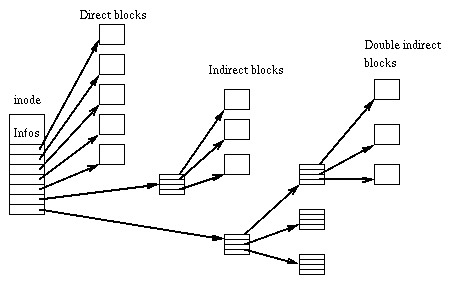
\includegraphics{Ext2-inode.jpg}
\end{center}

Luego un sistema de archivos será un conjunto (una tabla) de estos
nodos-i (estructuras) guardados dentro de la partición que contiene el 
sistema de archivos. 

\fcolorbox{black}{grey}{
\parbox[t]{1.0\linewidth}{ \vspace*{0.4cm}
{\bf 
Una conclusión que puede derivarse, es que 
el sistema de archivos en sí mismo consume espacio para almacenar las 
estructuras dentro del dispositivo de almacenamiento, lo cual debe ser 
tenido en cuenta a la hora de diseñar el tamaño del sistema de archivos. 
}
\vspace*{0.4cm} } }


\subsection*{Sistemas de archivos soportados por Linux}

Linux soporta una gran cantidad de tipos diferentes de sistemas de archivos. Para nuestros propósitos los más importantes son:

minix

    El más antiguo y supuestamente el más fiable, pero muy limitado en características (algunas marcas de tiempo se pierden, 30 caracteres de longitud máxima para los nombres de los archivos) y restringido en capacidad (como mucho 64 MB de tamaño por sistema de archivos).
xia

    Una versión modificada del sistema de archivos minix que eleva los límites de nombres de archivos y tamaño del sistema de archivos, pero por otro lado no introduce características nuevas. No es muy popular, pero se ha verificado que funciona muy bien.
ext3

    El sistema de archivos ext3 posee todas las propiedades del sistema de archivos ext2. La diferencia es que se ha añadido una bitácora (journaling). Esto mejora el rendimiento y el tiempo de recuperación en el caso de una caída del sistema. Se ha vuelto más popular que el ext2.
ext2

    El más sistema de archivos nativo Linux que posee la mayor cantidad de características. Está diseñado para ser compatible con diseños futuros, así que las nuevas versiones del código del sistema de archivos no necesitará rehacer los sistemas de archivos existentes.
ext

    Una versión antigua de ext2 que no es compatible en el futuro. Casi nunca se utiliza en instalaciones nuevas, y la mayoría de la gente que lo utilizaba han migrado sus sistemas de archivos al tipo ext2.
reiserfs

    Un sistema de archivos más robusto. Se utiliza una bitácora que provoca que la pérdida de datos sea menos frecuente. La bitácora es un mecanismo que lleva un registro por cada transacción que se va a realizar, o que ha sido realizada. Esto permite al sistema de archivos reconstruirse por sí sólo fácilmente tras un daño ocasionado, por ejemplo, por cierres del sistema inadecuados.

Adicionalmente, existe soporte para sistemas de archivos adicionales ajenos, para facilitar el intercambio de archivos con otros sistemas operativos. Estos sistemas de archivos ajenos funcionan exactamente como los propios, excepto que pueden carecer de características usuales UNIX , o tienen curiosas limitaciones, u otros inconvenientes.

msdos

    Compatibilidad con el sistema de archivos FAT de MS-DOS (y OS/2 y Windows NT).
umsdos

    Extiende el dispositivo de sistema de archivos msdos en Linux para obtener nombres de archivo largos, propietarios, permisos, enlaces, y archivos de dispositivo. Esto permite que un sistema de archivos msdos normal pueda utilizarse como si fuera de Linux, eliminando por tanto la necesidad de una partición independiente para Linux.
vfat

    Esta es una extensión del sistema de archivos FAT conocida como FAT32. Soporta tamaños de discos mayores que FAT. La mayoría de discos con MS Windows son vfat.
iso9660

    El sistema de archivos estándar del CD-ROM; la extensión popular Rock Ridge del estándar del CD-ROM que permite nombres de archivo más largos se soporta de forma automática.
nfs

    Un sistema de archivos de red que permite compartir un sistema de archivos entre varios ordenadores para permitir fácil acceso a los archivos de todos ellos.
smbfs

    Un sistema de archivos que permite compartir un sistema de archivos con un ordenador MS Windows. Es compatible con los protocolos para compartir archivos de Windows.
hpfs

    El sistema de archivos de OS/2.
sysv

    EL sistema de archivos de Xenix, Coherent y SystemV/386..

La elección del sistema de archivos a utilizar depende de la situación. Si la compatibilidad o alguna otra razón hace necesario uno de los sistemas de archivos no nativos, entonces hay que utilizar ése. Si se puede elegir libremente, entonces lo más inteligente sería utilizar ext3, puesto que tiene todas las características de ext2, y es un sistema de archivos con bitácora.

Existe también el sistema de archivos proc, generalmente accesible desde el directorio /proc, que en realidad no es un sistema de archivos, aún cuando lo parece. El sistema de archivos proc facilita acceder a ciertas estructura de datos del núcleo, como la lista de procesos (de ahí el nombre). Hace que estas estructuras de datos parezcan un sistema de archivos, y que el sistema de archivos pueda ser manipulado con las herramientas de archivos habituales. Por ejemplo, para obtener una lista de todos los procesos se puede utilizar el comando

{\tt
\$ ls -l /proc\\
total 0\\
dr-xr-xr-x   4 root     root            0 Jan 31 20:37 1\\
dr-xr-xr-x   4 liw      users           0 Jan 31 20:37 63\\
dr-xr-xr-x   4 liw      users           0 Jan 31 20:37 94\\
dr-xr-xr-x   4 liw      users           0 Jan 31 20:37 95\\
dr-xr-xr-x   4 root     users           0 Jan 31 20:37 98\\
dr-xr-xr-x   4 liw      users           0 Jan 31 20:37 99\\
-r--r--r--   1 root     root            0 Jan 31 20:37 devices\\
-r--r--r--   1 root     root            0 Jan 31 20:37 dma\\
-r--r--r--   1 root     root            0 Jan 31 20:37 filesystems\\
-r--r--r--   1 root     root            0 Jan 31 20:37 interrupts\\
-r--------   1 root     root      8654848 Jan 31 20:37 kcore\\
-r--r--r--   1 root     root            0 Jan 31 11:50 kmsg\\
-r--r--r--   1 root     root            0 Jan 31 20:37 ksyms\\
-r--r--r--   1 root     root            0 Jan 31 11:51 loadavg\\
-r--r--r--   1 root     root            0 Jan 31 20:37 meminfo\\
-r--r--r--   1 root     root            0 Jan 31 20:37 modules\\
dr-xr-xr-x   2 root     root            0 Jan 31 20:37 net\\
dr-xr-xr-x   4 root     root            0 Jan 31 20:37 self\\
-r--r--r--   1 root     root            0 Jan 31 20:37 stat\\
-r--r--r--   1 root     root            0 Jan 31 20:37 uptime\\
-r--r--r--   1 root     root            0 Jan 31 20:37 \\
version\\
\$\\
}

(Puede haber no obstante algunos archivos adicionales que no correspondan con ningún proceso. El ejemplo anterior se ha recortado.)

Tenga en cuenta que aunque se llame sistema de archivos, ninguna parte del sistema de archivos proc toca el disco. Existe tan sólo en la imaginación del núcleo. Cuando alguien intenta echar un vistazo a alguna parte del sistema de archivos proc, el núcleo hace que parezca como si esa parte existiera en alguna parte, aunque no lo haga. Así, aunque exista un archivo /proc/kcore de muchos megabytes, no quita espacio del disco.
¿Qué sistemas de archivos deben utilizarse?

Existe generalmente poca ventaja en utilizar muchos sistemas de archivos distintos. Actualmente, el más popular sistema de archivos es ext3, debido a que es un sistema de archivos con bitácora. Hoy en día es la opción más inteligente. Reiserfs es otra elección popular porque también posee bitácora. Dependiendo de la sobrecarga del listado de estructuras, velocidad, fiabilidad (percibible), compatibilidad, y otras varias razones, puede ser aconsejable utilizar otro sistema de archivos. Estas necesidades deben decidirse en base a cada caso.

Un sistema de archivos que utiliza bitácora se denomina sistema de archivos con bitácora. Un sistema de archivos con bitácora mantiene un diario, la bitácora, de lo que ha ocurrido en el sistema de archivos. Cuando sobreviene una caída del sistema, o su hijo de dos años pulsa el botón de apagado como el mío adora hacer, un sistema de archivos con bitácora se diseña para utilizar los diarios del sistema de archivos para recuperar datos perdidos o no guardados. Esto reduce la pérdida de datos y se convertirá en una característica estándar en los sistemas de archivos de Linux. De cualquier modo, no extraiga una falsa sensación de seguridad de esto. Como todo en esta vida, puede haber errores. Procure siempre guardar sus datos para prevenir emergencias.



\section*{Referencias}

[Intro] Tutuorial Introducción a la Administración de Sistemas GNU/Linux. Materia Introducción
a la Administración de Sistemas. UNCOMA. TUASSL. 

\section*{Licencia}

\end{document}
